%%!TEX root = ./UserManual.tex
\chapter{Software}
\label{chap:software}


%%%%%%%%%%%%%%%%%%%%%%%%%%%%%%%%%%%%%%%%%%%%%%%%%%%%%%%%%%%%%%%%
% System Requirements
%%%%%%%%%%%%%%%%%%%%%%%%%%%%%%%%%%%%%%%%%%%%%%%%%%%%%%%%%%%%%%%%
\section{System Requirements}
\label{section:system}

Indismo is written in C++ and portable over all platforms that have the GNU C++ compiler. 
De software has no dependencies on external libraries. The following tools needs to be installed:
\begin{compactitem}
    \item g++
    \item make
    \item CMake
    \item Python (optional, for automatization)
    \item Doxygen (optional, for documentation)
    \item LaTeX (optional, for documentation)
\end{compactitem}


%%%%%%%%%%%%%%%%%%%%%%%%%%%%%%%%%%%%%%%%%%%%%%%%%%%%%%%%%%%%%%%%
% Installation
%%%%%%%%%%%%%%%%%%%%%%%%%%%%%%%%%%%%%%%%%%%%%%%%%%%%%%%%%%%%%%%
\section{Installation}
\label{section:Installation}

To install the project, first obtain the source code by cloning the repository to a directory (e.g., ``git clone
https://bitbucket.org/indismo/indismo'') or download a zip file with all project
material from the Bitbucket website and de-compress the archive. 
The build system for indismo uses the CMake tool. This is used to build and install the software at a high level of abstraction and almost platform independent (see \url{http://www.cmake.org/}). 
The project includes the conventional make targets to ``build'', ``install'', ``test'' and ``clean'' the project. There is one additional target ``configure'' to set up the CMake/make structure that will actually do all the work.
For those users that do not have a working knowledge of CMake, a front end Makefile has been provided that invokes the appropriate CMake commands.
More details on building the software can be found in ``INSTALL.txt'' in the source folder.


%%%%%%%%%%%%%%%%%%%%%%%%%%%%%%%%%%%%%%%%%%%%%%%%%%%%%%%%%%%%%%%%
%
%%%%%%%%%%%%%%%%%%%%%%%%%%%%%%%%%%%%%%%%%%%%%%%%%%%%%%%%%%%%%%%
\section{Documentation}
\label{section:documentation}

The Application Programmer Interface (API) documentation is generated automatically using Doxygen from documentation instructions embedded in the code (see \url{www.doxygen.org}). 
The developer documentation is written in Doxygen syntax and can be generated in HTML format. Figure \ref{fig:doxygenapi} presents the home page of the API documentation.
The user manual distributed with the source code is written in \LaTeX (see \url{www.latex-project.org}).

\begin{figure}[h]
	\begin{center}
		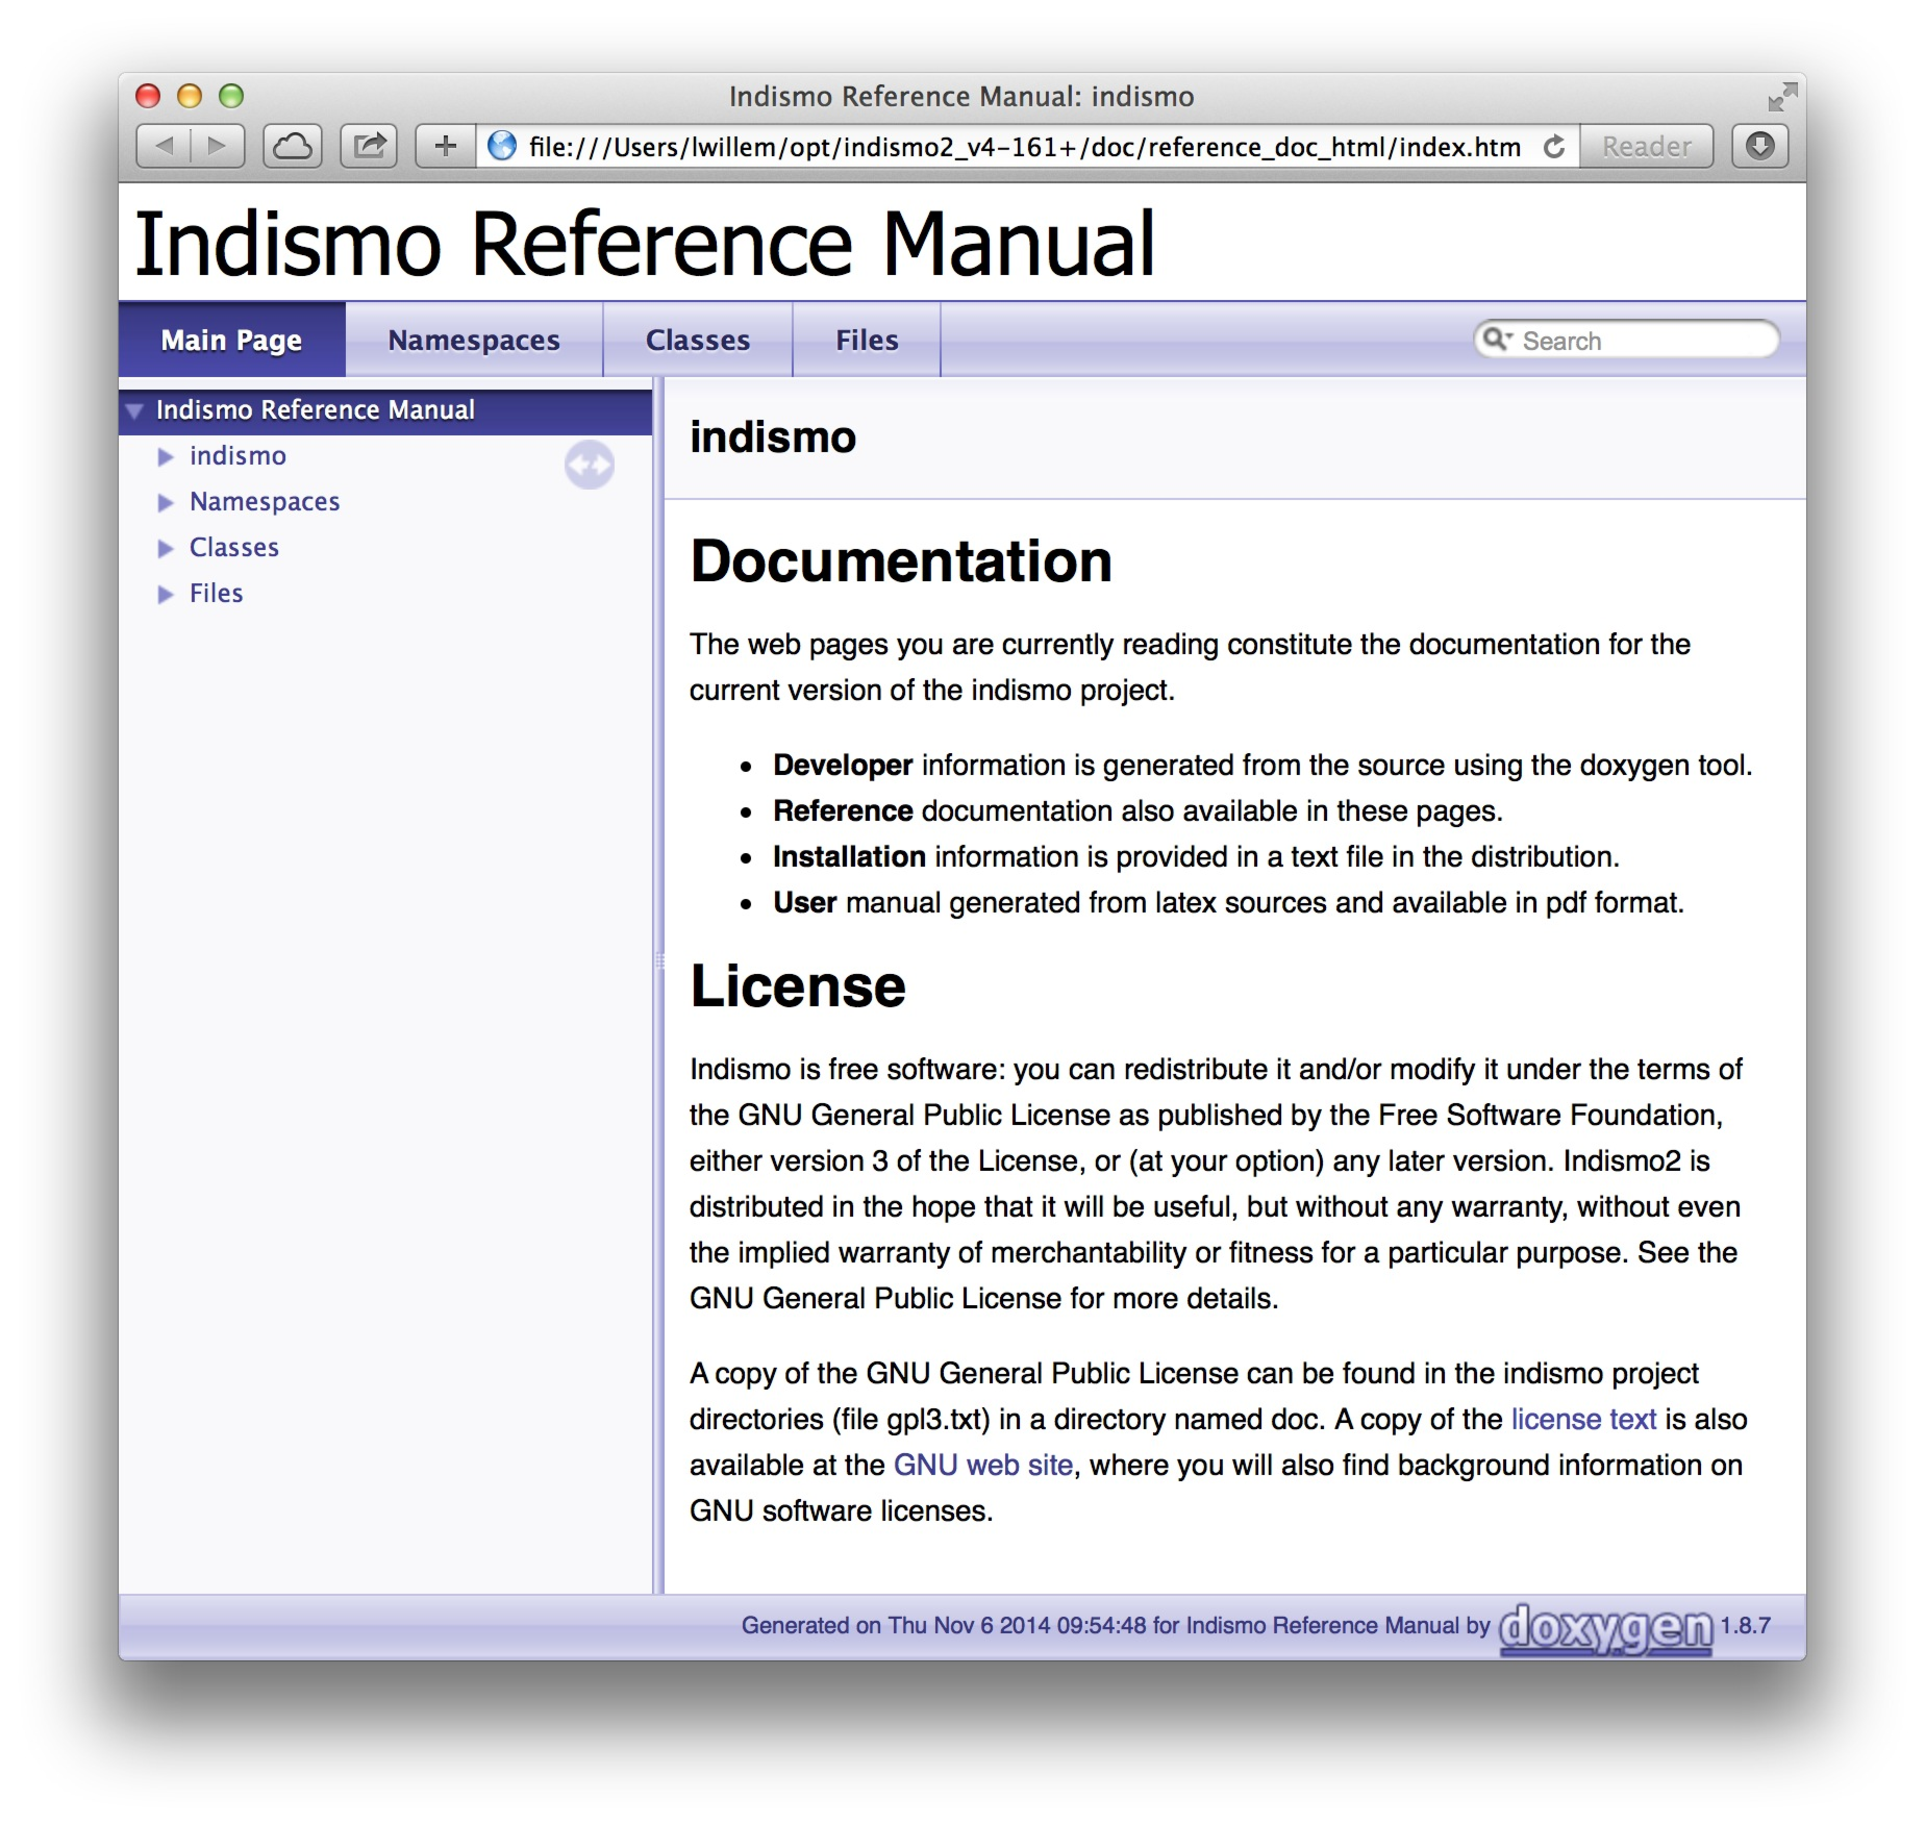
\includegraphics[width=0.8\textwidth]{images/screen_shot_doxygen_API.pdf}  
	\end{center}
	\caption{Screenshot of API documentation generated with Doxygen.}
	\label{fig:doxygenapi}
\end{figure}


%%%%%%%%%%%%%%%%%%%%%%%%%%%%%%%%%%%%%%%%%%%%%%%%%%%%%%%%%%%%%%%%
%
%%%%%%%%%%%%%%%%%%%%%%%%%%%%%%%%%%%%%%%%%%%%%%%%%%%%%%%%%%%%%%%
\section{Directory layout}

The project directory structure is designed following maven conventions.
Everything used to build the software is stored in directory \texttt{./src}:
\begin{compactitem}
    \item \texttt{src/main}: Code related files (sources, third party libraries and headers, ...)
      	\begin{itemize}
        		\item \texttt{src/main/"language"}: source code, per coding language 
        		\item \texttt{src/main/resources}: third party resources
        \end{itemize}
    \item \texttt{src/doc}: documentation files (API, manual, ...)
      	\begin{itemize}
        		\item \texttt{src/doc/"tool"}: files per document processing tools
        \end{itemize}
    \item \texttt{src/test}: test related files (scripts, regression files, ...)
\end{compactitem}
Every artefact during the build procedure is generated in directory \texttt{./target} and is completely removed when the project is cleaned.

%%%%%%%%%%%%%%%%%%%%%%%%%%%%%%%%%%%%%%%%%%%%%%%%%%%%%%%%%%%%%%%%
% File formats
%%%%%%%%%%%%%%%%%%%%%%%%%%%%%%%%%%%%%%%%%%%%%%%%%%%%%%%%%%%%%%%%
\section{File formats}
\label{section:FileFormats}

The indismo software supports two file formats: 
\begin{description}
	\item [CSV] \ \\
	Comma separated values, used for population input data and the simulator output.
	\item [JSON] \ \\
	JavaScript Object Notation, an open standard format that uses human-readable text to transmit objects consisting of attribute-value pairs. 	 \mbox{(see \url{www.json.org})}
\end{description}


%%%%%%%%%%%%%%%%%%%%%%%%%%%%%%%%%%%%%%%%%%%%%%%%%%%%%%%%%%%%%%%%
%
%%%%%%%%%%%%%%%%%%%%%%%%%%%%%%%%%%%%%%%%%%%%%%%%%%%%%%%%%%%%%%%%
\section{Testing}
Unit tests and install checks are added to indismo based on Google's ``gtest" framework and CMake's ``ctest" tool. 
In addition, the code base contains assertions to verify the simulator logic. 
They are activated when the application is built in debug mode and can be used to catch errors at run time. 




%%%%%%%%%%%%%%%%%%%%%%%%%%%%%%%%%%%%%%%%%%%%%%%%%%%%%%%%%%%%%%%%
% Results
%%%%%%%%%%%%%%%%%%%%%%%%%%%%%%%%%%%%%%%%%%%%%%%%%%%%%%%%%%%%%%%%
\section{Results}
\label{section:Results}

The software generates two output files:
\begin{description}
	\item [Log] \ \\
	Cumulative number of cases per day.
	\item [Output] \ \\
	Aggregated results on the number of cases, configuration details and timings.
\end{description}	
	
	
	
